\subsection{Accelerometer algortime}\label{sec:imp_vinkler}
I \autoref{sec:test_acc} fremgår det, at der er lineær sammenhæng mellem vinkel og spænding. Det er derfor muligt at udføre en lineær interpolation over dataen af målinger fra accelerometrene i forskellige vinkler. På denne måde er det muligt at bestemme, hvilken som helst vinkel for en tilsvarende spænding. 
%Da målingerne af linearitet, målt i \autoref{sec:test_acc}, er foretaget med Ni USB-6009 stemmer spændingerne ikke overens, når det samples på mikrokontrolleren. Dette gør det ikke, da Ni USB-6009 og mikrokontrolleren har forskellige arbejdsområder,
Derfor udføres der en ny måling af linearitet med mikrokontrolleren, hvor spændingen i de forskellige vinkler er målt. Efterfølgende er der aflæst et offset, som er trukket fra, for at centrere signalet omkring 0. Offsettet for accelerometeret placeret på låret er aflæst til $1002$, hvilket svarer til et offset på $1,6162~V$ og accelerometeret placeret på skinnebenet til $972$, svarende til et offset på $1,5743~V$. Det digitale output ved forskellige vinkler fremgår af \autoref{tab:vinkelinterval_psoc}. Disse digitale output er omregnet til en spænding ved \autoref{eq:vinkler}, hvor $3,3~V$ er forsyningsspændingen, og $2^{11}$ er ADC'ens oplæsning målt i bits.  

\begin{equation}
\label{eq:vinkler}
sp\text{æ}nding =digitalt~output\cdot \dfrac{3,3~V}{2^{11}}
\end{equation}

\noindent
Resultaterne for de nye målinger fremgår af \autoref{tab:vinkelinterval_psoc}, hvor det konverteret output for accelerometrene på henholdsvis låret og skinnebenet er angivet som en vinkel på 0, 10, 30, 50, 70, 80 og $90^{\circ}.$ 

\begin{table}[H]
\centering
\begin{tabular}{|c|c|c|}
\hline
\multicolumn{1}{|l|}{\textbf{Vinkel {[}$^{\circ}${]}}} & \textbf{\begin{tabular}[c]{@{}c@{}}Konverteret output fra acclerometer \\ placeret på låret\end{tabular}} & \textbf{\begin{tabular}[c]{@{}c@{}}Konverteret output fra accelerometer \\ placeret på skinnebenet\end{tabular}} \\ \hline
0                                                      & -186                                                                                                     & -179                                                                                                            \\ \hline
10                                                     & -185                                                                                                   & -176
\\ \hline
30                                                     & -168                                                                                                   & -153                                                                                                          \\ \hline
50                                                     & -126                                                                                                  & -111                                                                                                         \\ \hline
70                                                     & -76                                                                                                  & -52                                                                                                         \\ \hline
80                                                     & -31                                                                                                  & -16                                                                                                         \\ \hline
90                                                     & 0
& 0
\\ \hline
\end{tabular}
\caption{Konverteret output fra accelerometer placeret på låret og på skinnebenet svarende til en given spænding.}
\label{tab:vinkelinterval_psoc}  
\end{table}


Ud fra de målte værdier i \autoref{tab:vinkelinterval_psoc}, er der opstillet en funktion indeholdt \textit{ifelse}-løkker, hvorved det er muligt at vurdere, hvilket interval en given spænding befinder sig indenfor. I hver enkelt løkke anvendes lineær interpolation, som har til opgave at finde en vinkel, der er svarende til en spænding som ligger mellem et interval og returnerer denne. 

Når der er udført lineær interpolation over dataen skal de målte data fra låret samt skinnebenet ligges sammen for at få den samlede vinkel over knæet under squat-øvelsen. Denne øvelse er beskrevet i \autoref{sec:knaeled_squat}.
Ved at implementere værdierne fra \autoref{tab:vinkelinterval_psoc} kan signalet repræsenteres som samlet grader over tid, som det ses af \autoref{fig:acc_imp}.
 

\begin{figure}[H]
\centering
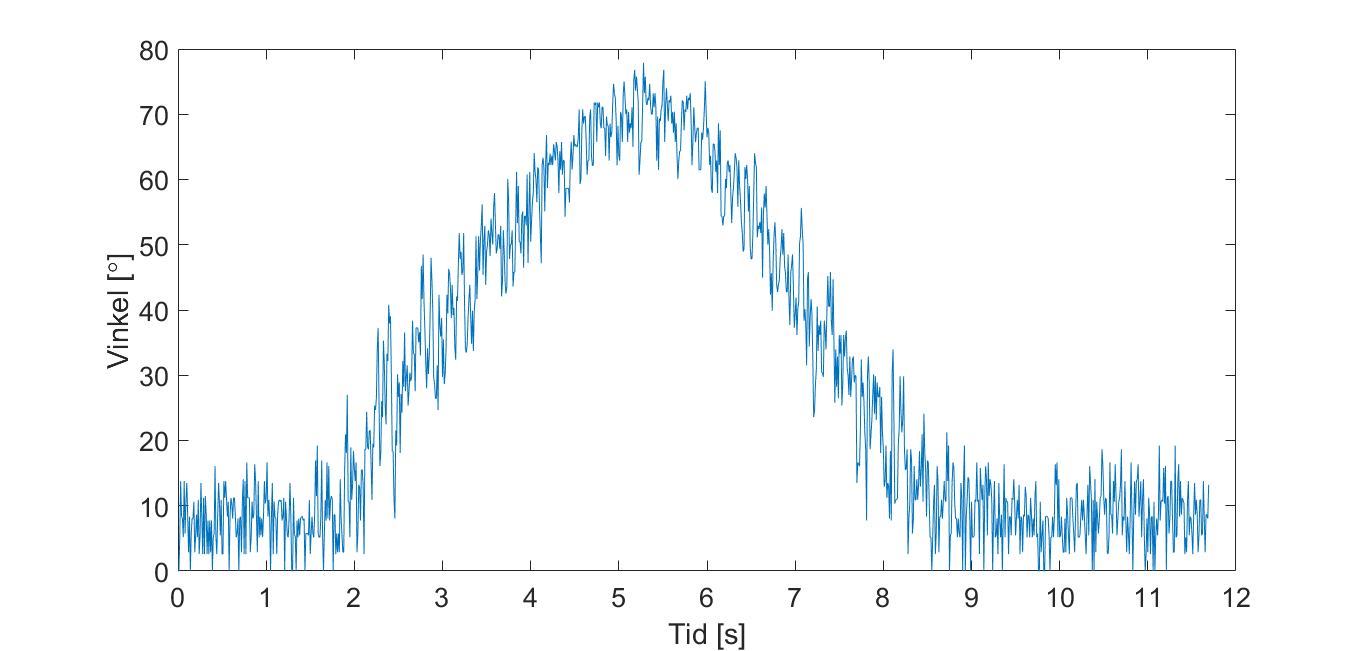
\includegraphics[width=0.8\textwidth]{figures/Pilotforsoeg/accvinkel}
\caption{Samlet vinkler af accelerometrene under udførelse af squat-øvelsen, der er defineret i \autoref{sec:knaeled_squat}.}
\label{fig:acc_imp}
\end{figure}



